\chapter{Technologie}\label{ch:technology}

Um die Verwendungszwecke von Docker Swarm näher zu untersuchen, muss zunächst die grundlegende Technologie grob erläutert werden. 
Docker ist an sich eine open-source ``platform for developing, shipping, and running applications''\cite{DockerInc} und besteht aus mehreren Komponenten. 

\section{Architektur}

Aufgebaut ist Docker nach der Client-Server-Architektur. Der Client kann hierbei jede Maschine sein, auf der Docker oder Docker Compose installiert ist und die docker-Befehle ausf\"uhren kann. 
Auf der Server-Seite steht dem gegen\"uber der Docker Daemon, der die eigentlichen Aufgaben des Bauens und Auslieferns \"ubernimmt. 
Ein Client kann dabei mit mehreren Daemons \"uber die Docker API kommunizieren. 

\begin{figure}[h]
    \centering
    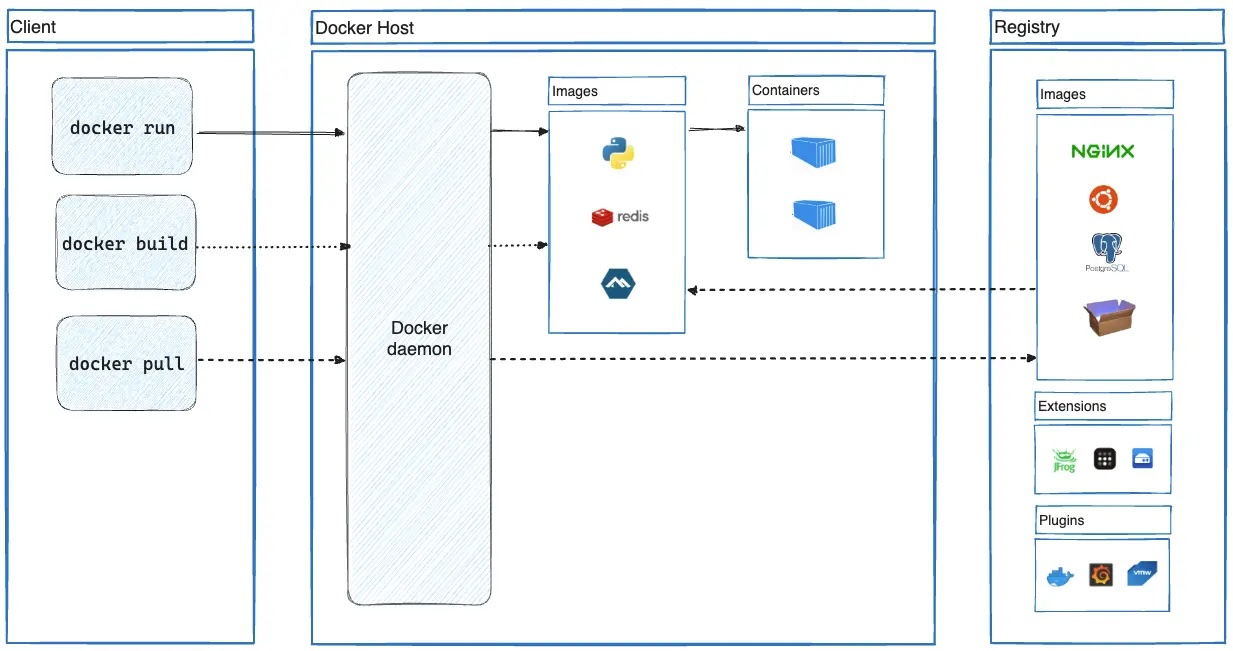
\includegraphics[width=0.7\textwidth]{figures/docker-architecture.jpeg}
    \caption{Aufbau der Docker-Architektur\cite{DockerInc}}
    \label{fig:docker-architecture}
\end{figure}

F\"ur Enduser-Betriebssysteme ist hier die Docker Desktop-Software relevant, die den Client, Daemon, Docker Compose  und weitere hilfreiche Komponenten mit einer graphischen Oberfl\"ache zusammen verpackt. 
Die dritte wesentliche Rolle neben Client und Daemon spielen die sogenannten Docker Registries, in denen Docker Images gespeichert werden. 
Docker selbst stellt eine \"offentliche Registry zur Verf\"ugung, das Docker Hub, in der viele offizielle Images wie bspw.\ die Base-Images f\"ur Datenbanken wie postgres, Reverse Proxys wie traefik oder auch simple Testimages wie hello-world zu finden sind. 
Dar\"uber hinaus kann jeder registrierte User dort kostenlos ein privates Repository sowie unbegrenzt viele \"offentliche Repositories f\"ur eigene Images erstellen. 
Unternehmen und Hochschulen verwenden hingegen in der Regel ein eigenes privates Registry, wenn die Images der Allgemeinheit nicht (kostenlos) zur Verf\"ugung gestellt werden soll.

Im Folgenden sollen zwei essentielle Aspekte beleuchtet werden; zum einen der grundlegende Aufbau und die Funktionalit\"at von Docker Containern und zum anderen das Konzept der Containerorchestrierung.

\section{Docker Container}

Docker Container basieren auf der Linux Container-Technologie und stellen eine Abstraktionsebene der klassischen Infrastruktur dar. 
W\"ahrend sie theoretisch als Alternative zur herkömmlichen Virtualisierung von Servern zum Einsatz kommen k\"onnen, werden diese beiden Technologien in der Praxis meist kombiniert. 
Das Ziel ist dabei, eine Umgebung zu schaffen, die dem gewünschten Betriebssystem möglichst nah kommt, ohne einen separaten Kernel zu benötigen\cite{quan_connecting_2016} und dabei gleichzeitig leichtgewichtig und portabel genug zu sein, um jederzeit schnell und bestenfalls automatisiert ersetzt werden zu k\"onnen. 
Container verpacken Software in einem vollständigen Dateisystem, das alles beinhaltet, was gebraucht wird, um die Software zuverlässig und konsistent  auszuführen. 
Das umfasst sowohl den Code als auch die Laufzeitumgebung, Bibliotheken und weitere Abhängigkeiten.\cite{nguyen_distributed_2017}
Sie bestehen also ``aus einem oder mehreren Prozessen, die vom Rest des Systems isoliert sind''.\cite{red_hat_was_2023}
Die Isolation des Codes gegen\"uber anderen Containern auf dem gleichen System wird gew\"ahrleistet, indem die Docker Engine f\"ur jeden Container einen eigenen Namespace erstellt, an den alle Aspekte des Containers gebunden sind.\cite{DockerInc}
Im Gegensatz zu Kubernetes findet dies aber nur intern statt und wird nicht durch die Anwenderin direkt beeinflusst. 

\begin{figure}[h]
    \centering
    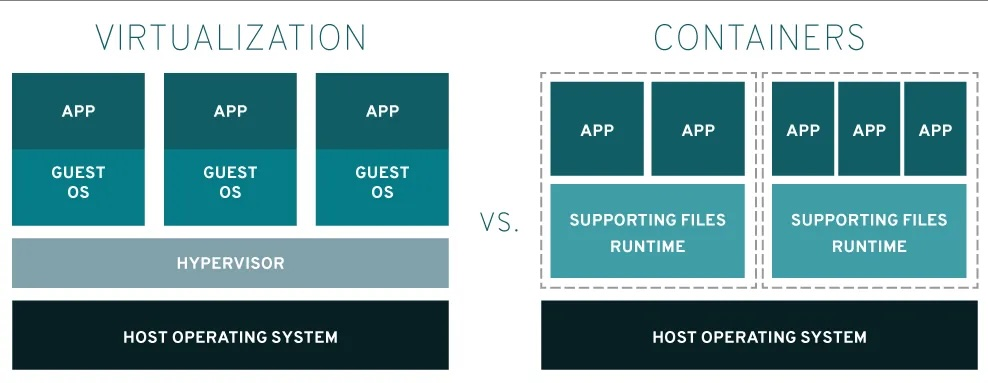
\includegraphics[width=0.7\textwidth]{figures/virtualization-vs-containers.jpeg}
    \caption{Vergleich von Virtualisierung und Containerisierung\cite{red_hat_was_2023}}
    \label{fig:virtualization-comparison}
\end{figure}

Im Gegensatz zur Virtualisierung, bei der für jede virtuelle Maschine ein eigenes Betriebssystem installiert wird, verwendet die Containerisierung das Betriebssystem des Hosts, wodurch die Container leichtgewichtiger und portabler sind. 
Im Umkehrschluss bedeutet das aber auch, dass ein Container immer nur auf dem Betriebssystem laufen kann, für das er gebaut wurde. 
So kann ein Container mit einer zugrunde liegenden ARM-Architektur nicht auf einem x86 Linux-System laufen und umgekehrt. 
Da es aber möglich ist, die Zielarchitektur beim Erstellen zu definieren, stellt dies in der Praxis kein echtes Problem dar.

\section{Docker Images}

``Alle zur Ausführung [eines Containers] notwendigen Dateien werden über ein eigenes Image bereitgestellt''\cite{red_hat_was_2023}, das in einer Textdatei namens Dockerfile beschrieben ist. 
Das Image stellt somit eine Vorlage für die einzelnen Container dar, die die Docker Engine instanziiert. 
Es basiert in der Regel auf einem vorgefertigten Image, wie bspw.\ node als Laufzeitumgebung zum Bauen des Codes und nginx als Webserver zum Ausliefern im Codebeispiel~\ref{lst:Dockerfile}.
Die Datei besteht aus Instruktionen, die sequentiell abgearbeitet werden, wobei jede Instruktion ein Layer des Images erstellt.
Daher werden beim Bauen eines Images nur diejenigen Layer neu gebaut, in denen sich etwas ge\"andert hat.

\lstinputlisting[language=bash,caption={Codebeispiel eines Dockerfiles},captionpos=b,label=lst:Dockerfile]{listings/Dockerfile}

Wird nun auf Basis des erstellten Images ein Container erstellt, verändern die Instruktionen das Dateisystem der jeweiligen Laufzeitumgebung, aber immer nur in Bezug auf den Namespace des Containers. 
